% feasibility-report.tex: 可行性报告
% Copyright (C) 2022 吴骏东, 张子辰, 蓝俊玮, 郭耸霄 and 陈建绿
% All rights reserved.

% This file is part of Runikraft. Runikraft is free software,
% which is released under the BSD 3-Clause License, see LICENSE for details.
% Runikraft is provided ``as is'', without any express or implied warrenties.

% The reports of Runikraft are released under the Creative Commons
% Attribution 4.0 International License; see report/LICENSE for details.
\documentclass[UTF8,fontset=none,linespread=1.15]{ctexart}
\ctexset
{
    section/format={\Large\sffamily\bfseries},
    subsection/format+={\sffamily},
    subsubsection/format+={\itshape}
}
\setCJKmainfont[ItalicFont={KaiTi},BoldItalicFont={KaiTi},
BoldItalicFeatures={FakeBold=3}]{Noto Serif CJK SC}
\setCJKsansfont[BoldFont={Noto Sans CJK SC Bold},
BoldItalicFont={Noto Sans CJK SC Bold},
AutoFakeSlant]{Noto Sans CJK SC DemiLight}
\setCJKmonofont[AutoFakeBold=3,AutoFakeSlant]{FangSong}
\setmainfont{cmun}[Extension=.otf,UprightFont=*rm,
ItalicFont=*ti,BoldFont=*bx,BoldItalicFont=*bi]
\setsansfont{cmun}[Extension=.otf,UprightFont=*ss,
ItalicFont=*si,BoldFont=*sx,BoldItalicFont=*so]
\setmonofont{cmun}[Extension=.otf,UprightFont=*btl,
ItalicFont=*bto,BoldFont=*tb,BoldItalicFont=*tx]
%Computer Modern Unicode 的\textasciitilde和\~{}的高度相同,所以用\tildechar表示居中的波浪线~
\newcommand{\tildechar}{\raisebox{-0.35em}{\textasciitilde}}
\usepackage[a4paper,hmargin=1.2in,vmargin=1in]{geometry}
\usepackage{graphicx,tikz,float,multicol,makecell,multirow,longtable}
\usepackage{verbatim}
\usepackage[normalem]{ulem}
\usepackage{CJKfntef}
\usepackage[perpage]{footmisc}

%目录, 参考了OSH-2021/x-sBPF
\usepackage{titletoc}
\titlecontents{section}[2em]{\addvspace{1.3mm}\bfseries}{%
\contentslabel{2.0em}}{}{\titlerule*[5pt]{$\cdot$}\contentspage}
\titlecontents{subsection}[4.2em]{}{\contentslabel{2.5em}}{}{%
\titlerule*[5pt]{$\cdot$}\contentspage}
\titlecontents{subsubsection}[7.2em]{}{\contentslabel{3.3em}}{}{%
\titlerule*[5pt]{$\cdot$}\contentspage}

%图表标题
\usepackage{caption}
\captionsetup{font={sf}}

%代码环境
\usepackage{listings}
\lstset{basicstyle={\normalfont\ttfamily},breaklines,tabsize=4}
\renewcommand{\lstlistingname}{代码}
\renewcommand{\lstlistlistingname}{代码}
%Rust
\lstdefinelanguage{Rust}
{
    morekeywords={as,async,await,break,const,continue,crate,dyn,else,enum,extern,false,fn,for,if,impl,in,let,loop,match,mod,move,mut,pub,ref,return,Self,self,static,struct,super,trait,true,type,union,unsafe,use,where,while,abstract,become,box,do,final,macro,override,priv,try,typeof,unsized,virtual,yield},
    sensitive=true,
    morecomment=[l]{//},
    morecomment=[s]{/*}{*/},
    morestring=[b]{"},
    morestring=[b]{'}
}


\usepackage{enumitem}
\setlistdepth{5}
\renewlist{enumerate}{enumerate}{5}
\setlist{itemsep=0pt,partopsep=0pt,parsep=0pt,topsep=0pt}
\setlist[enumerate,1]{label=\arabic*.}
\setlist[enumerate,2]{label=(\arabic*)}
\setlist[enumerate,3]{label=\textcircled{\arabic*}}
\setlist[enumerate,4]{label=(\textit{\roman*})}
\setlist[enumerate,5]{label=\textit{\alph*})}

\usepackage[colorlinks,unicode,pdfstartview={FitH}]{hyperref}
\hypersetup
{
  pdftitle={2022春 操作系统原理与设计(H) x-runikraft小组 可行性报告},
  pdfauthor={吴骏东; 张子辰; 蓝俊玮; 郭耸霄; 陈建绿}
}

%带圈数字,它必须在hyperref之后载入
\usepackage{xunicode-addon}
\makeatletter
\xeCJKDeclareCharClass{CJK}{"24EA, "2460->"2473, "3251->"32BF,"24B6->"24E9,"2160->"217F}
\newfontfamily\EnclosedNumbers{Noto Serif CJK SC}
\AtBeginUTFCommand[\textcircled]{\begingroup\EnclosedNumbers}
\AtEndUTFCommand[\textcircled]{\endgroup}
\makeatother

\makeatletter
\let\textcircled@old\textcircled
\protected\def\textcircled#1{%
	\expandafter\textcircled@old\expandafter{\expanded{#1}}}
\makeatother
\makeatletter
\renewcommand\@makefntext[1]{%
	\setlength\parindent{0.75\ccwd}\selectfont
	\@thefnmark\ #1}
\makeatother
\renewcommand*\thefootnote{\textcircled{\arabic{footnote}}}
\renewcommand{\lstlistingname}{代码}

%上标+引用
\let\nosupcite\cite
\renewcommand*{\cite}[1]{\textsuperscript{\nosupcite{#1}}}

%章节作者
\newcommand{\sectionauthor}[1]{%
\vspace*{-5ex}
\noindent\textrm{\hfill\textit{by #1}}
\vspace*{2ex}\par}
%\renewcommand{\today}{2022年4月5日}

\begin{document}
\sffamily %为方便屏幕阅读,文档主要使用无衬线字体
\title{\bfseries Runikraft小组\quad 可行性报告}
\author{吴骏东\and 张子辰\and 蓝俊玮\and 郭耸霄\and 陈建绿}
\date{\today}
\maketitle

\tableofcontents

\section{理论依据}
我们的项目的可行性要点在于使用Rust语言改写与基于RISC-V架构开发,这两个新事物都有很多优点,而且已经有了很多应用。为了实现一个安全的Unikernel,在理论部分还需要考虑程序设计语言保证内存和线程安全的方式,以及架构对特权指令的支持。

Rust 所拥有的语言特性,使得它能够保证内存安全和线程安全,而且它的速度和C/C++同级;同时 Rust 支持与外部代码进行交互以及 unsafe Rust,这也增加了它的灵活性。因此我们可以自信地说,使用 Rust 编写操作系统是十分可行的。

\textbf{Rust Language}

A language empowering everyone to build reliable and efficient software.\cite{7}用Rust改写项目已经成为一种解决问题的有效手段,如zalando公司从Scala转向Rust的成功故事。\cite{3}

\textbf{RISC-V Architecture}

RISC-V is a free and open ISA enabling a new era of processor innovation through open standard collaboration.\cite{0}目前基于RISC-V架构的开源处理器有很多,既有标量处理器Rocket,也有超标量处理器BOOM,还有面向嵌入式领域的Z-scale、PicoRV32等。\cite{2}
\subsection{Rust保证内存安全的方式}
在高级语言中,某个内存位置要在程序中能被访问,必然就会与一个或多个变量建立关联关系。这会引出内存的不正确访问引发的内存安全问题。这些问题在C/C++中都是需要开发者非常小心地自己处理。而 Rust 的语言特性则为上面的问题提供了解决方案。\cite{8}
\begin{table}[H]
\centering
\caption{Rust对内存安全问题的解决方案}
\begin{tabular}{|c|c|}
\hline
\textbf{问题} & \textbf{Rust 的解决方案}\\\hline
使用未初始化内存&编译器禁止变量读取未赋值变量\\\hline
对空指针解引用&使用\texttt{Option}枚举替代空指针\\\hline
悬垂指针&生命周期标识与编译器检查\\\hline
缓冲区溢出&编译器检查,拒绝超越缓冲区边界的数据访问\\\hline
非法释放内存&语言级的 RAII 机制,唯一的所有者才有权释放内存\\\hline
\end{tabular}
\end{table}
\subsection{Rust保证线程安全的方式}
Rust 通过一整套设计非常精良的基础设施来保证这一点,这些基础设施配合类型检查和借用模型“强迫”程序员写出正确的代码,把别的语言在运行时的崩溃或泄露暴露在编译期,从而保证线程安全。

\textbf{基础设施}

1. 进行语义限制的\texttt{Send} / \texttt{Sync} 、\texttt{Trait}。

2. 共享不可变所有权的\texttt{Arc} (\texttt{Rc}的多线程版本)。

3. 提供内部可变性的\texttt{Mutex} / \texttt{Rwlock}。

4. 管道模型\texttt{channel}。

5. 其他的一些线程相关的API。

\textbf{线程相关的常见API与设施}

1. \texttt{std::thread::spawn},\texttt{spawn}接收一个闭包并执行,返回一个\texttt{JoinHandle}类型的值,它拥有线程所有权;

2. \texttt{join()}函数,该函数作用在线程句柄\texttt{JoinHandle}类型的值上,使得父线程能够等待子线程执行完毕;

3. \texttt{move}+闭包,\texttt{move}闭包常常与\texttt{thread}和\texttt{spawn}一起使用,它允许我们在一个线程中使用另外一个线程的数据,使用\texttt{move}关键字强制闭包获取其使用的环境值的所有权。

Rust 所拥有的这些设施以及自身的特性可以让我们编写出正确的代码从而保证线程安全。\cite{9}

\subsection{RISC-V对特权指令的支持}
截至目前(2022.4),RISC-V 共定义了四个特权级别,由高到低排列顺次为:

\textbf{机器级别(M)}:RISC-V中硬件线程可以执行的最高权限模式。在M模式下运行的 hart 对内存、I/O 和一些对于启动和配置系统来说必要的底层功能有着完全的使用权。因此它是唯一所有标准 RISC-V 处理器都必须实现的权限模式。\cite{a}

\textbf{超级监管者级别(H)}:为了支持虚拟机监视器。但目前该级别并没有被正式加入到文档中。

\textbf{监管者级别(S)}:为了支持现代类 Unix 操作系统,如 Linux , FreeBSD 和 Windows 。

\textbf{用户级别(U)}:用于运行应用程序,适用于安全嵌入式系统。

标准的 RISC-V 为超过4000个 CSR 预留了12位的编码空间([11:0])。其中,[11:8] 位根据特权级别对 CSR 的读写权限进行编码。注意:任何试图访问不存在的 CSR 的行为均会引发指令异常,尝试写入只读寄存器也会引发指令异常。剩余的8位编码 [7 :  0] 将指定相应的寄存器地址位置。具体细节如下所示:\cite{b}\cite{c}

\begin{lstlisting}[numbers=left]
CSR [11:10]:对读写模式进行约束
00		read/write
01		read/write
10		read/write
11		read-only
CSR [9:8]:对访问最低权限进行约束
00		Unprivileged and User-Level CSRs
01		Supervisor-Level CSRs
10		Hypervisor and VS CSRs
11		Machine-Level CSRs
\end{lstlisting}
除目前 RISC-V 支持的特权指令格式外,\texttt{ECALL}指令在Linux中用于系统调用。如下为\texttt{arch/riscv/kernel/sbi.c}中的部分代码,使用\texttt{ECALL}指令时,将异常类型写在a7 寄存器, 参数写在 a0-a5 寄存器,后面会根据异常类型的不同调用不同的异常处理函数。
​		例如实现一个putchar函数用于打印一个字符到系统控制台上,就如下通过ECALL来实现:
\begin{lstlisting}[numbers=left]
void sbi_console_putchar(int ch)
{
	sbi_ecall(SBI_EXT_0_1_CONSOLE_PUTCHAR, 0, ch, 0, 0, 0, 0, 0);
}
\end{lstlisting}
\section{技术依据}
我们的项目是使用 Rust 改写 Unikraft,来实现一个Unikernel。而 Unikraft 是使用 C 编写的,故我们在实现的过程中可能会因为某些原因保留少部分 C 代码,因此需要在 Rust 中调用这部分外部代码,即要实现 Rust 与 C 的交互。由于RISC-V开发板难以获得,我们决定在虚拟环境上搭建RISC-V架构。KVM恰满足了我们的需求。为了更方便地运行与调试KVM程序,我们决定使用QEMU。
\subsection{Rust与C交互}
Rust 中提供了\texttt{extern}关键字来简化创建和使用外部接口(Foreign Function Interface, FFI)的过程。FFI 是编程语言定义函数的一种方式,它允许其他(外部的)编程语言来调用这些函数。
下面是一个集成了C标准库中的\texttt{abs}函数的示例代码:
\begin{lstlisting}[numbers=left]
extern "C" {
	fn abs(input: i32) -> i32;
}
fn main(){
	unsafe {
		println!("Absolue value of -3 according to C: {}", abs(-3));
	}
}
\end{lstlisting}
这段代码在\texttt{extern "C"}块中列出了它想要调用的外部函数和签名,其中的\texttt{"C"}指明了外部函数使用的应用二进制接口(Application Binary Interface, ABI):它被用来定义函数在汇编层面的调用方式。

要在其他语言中调用 Rust 函数,同样可以使用\texttt{extern}来创建一个允许其他语言调用 Rust 函数的接口。创建时需要将\texttt{extern}关键字及对应的 ABI 添加到函数签名的\texttt{fn}关键字前,并为该函数添加\texttt{\#[no\_mangle]}注解来避免 Rust 在编译时改变它的名称。下面是一个可以在编译并链接后被 C 语言代码访问的函数定义:
\begin{lstlisting}[numbers=left]
#[no_mangle]
pub extern "C" fn call_from_c() {
	println!("Just called a Rust function from C!");
}
\end{lstlisting}
这一类型的\texttt{extern}功能不需要使用\texttt{unsafe}。
\subsection{KVM对RISC-V架构的支持}
KVM (Kernel-based Virtual Machine,基于内核的虚拟机)  ,是一种内建于 Linux 中的开源虚拟化技术。具体而言,KVM 可以将 Linux 转变为虚拟监控程序,从而使主机计算机能够运行多个隔离的虚拟环境,即虚拟客户机或虚拟机(VM)。
\begin{figure}[!hbt]
	\centering
	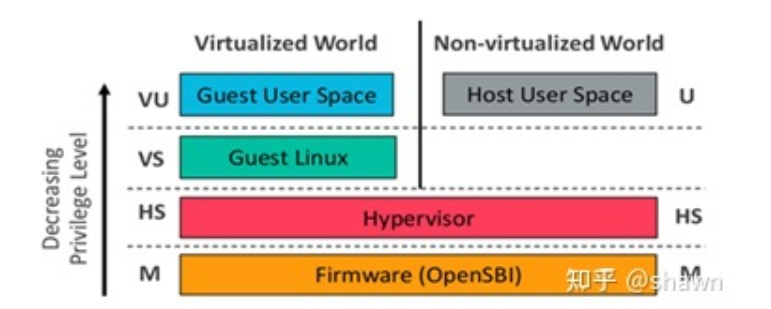
\includegraphics[width=0.7\linewidth]{assets/W4}
	\caption{虚拟化下的特权等级}
	\label{fig:w4}
\end{figure}

如图\ref{fig:w4},为了支持虚拟化,RISC-V 规范定义了 RISC-V H-extension ,在原来的3级特权架构的基础上对原有的 Supervisor 模式进行了扩展,引入了 Hypervisor-Extended Supervisor mode(HS)。此时,在 Machine Mode 下运行最高优先级的、对全部资源具备操作能力的 Firmware ,虚拟机软件 Hypervisor 运行在 HS 模式,虚拟机 VM 运行在虚拟化的 Supervisor 模式,应用程序继续运行在虚拟操作系统之上,运行在 Virtualized User mode。

为了实现 Supervisor 与 Hypervisor-extended supervisor 模式的切换,RSIC-V 将原来 Supervisor 模式下的 CSR 复制一份到Hypervisor,从而让每个硬件线程拥有两份 supervisor 寄存器,加快两个模式之间的切换过程。

由于 RISC-V 没有为不同虚拟化软件设计专门的特权模式,而是设计了统一的特权模式,这说明它对 1类(如Xvisor)、 2类(如KVM)虚拟化软件都有很好的支持。 RISC-V 可以通过 CSR 寄存器注入中断,因此不需要为虚拟化而特殊设计中断控制器外设。此外,RISC-V 可直接借助特殊的寄存器位支持嵌套虚拟化,而 Aarch64 要等到 v8.3 版本之后才支持这个功能。RISC-V 的时钟和核间中断可通过 SBI 软件辅助完成,而 Aarch64 需要特殊设计的计时器外设来支持虚拟化功能。\cite{d}
\subsection{QEMU}

QEMU is a generic and open source machine emulator and virtualizer.

When used as a machine emulator, QEMU can run OSes and programs made for one machine (e.g. an ARM board) on a different machine (e.g. your own PC). By using dynamic translation, it achieves very good performance.

When used as a virtualizer, QEMU achieves near native performance by executing the guest code directly on the host CPU. QEMU supports virtualization when executing under the Xen hypervisor or using the KVM kernel module in Linux. When using KVM, QEMU can virtualize x86, server and embedded PowerPC, 64-bit POWER, S390, 32-bit and 64-bit ARM, and MIPS guests.\cite{1}

\textbf{QEMU具有如下优点:}

\paragraph{Full-system emulation}Run operating systems for any machine, on any supported architecture.

\paragraph{User-mode emulation}Run programs for another Linux/BSD target, on any supported architecture.

\paragraph{Virtualization}Run KVM and Xen virtual machines with near native performance.\cite{1}

\section{创新点}
\section{概要设计}
Runikraft的架构与Unikraft几乎相同。
\begin{figure}[!hbt]
\centering
\begin{minipage}{0.49\linewidth}
\centering
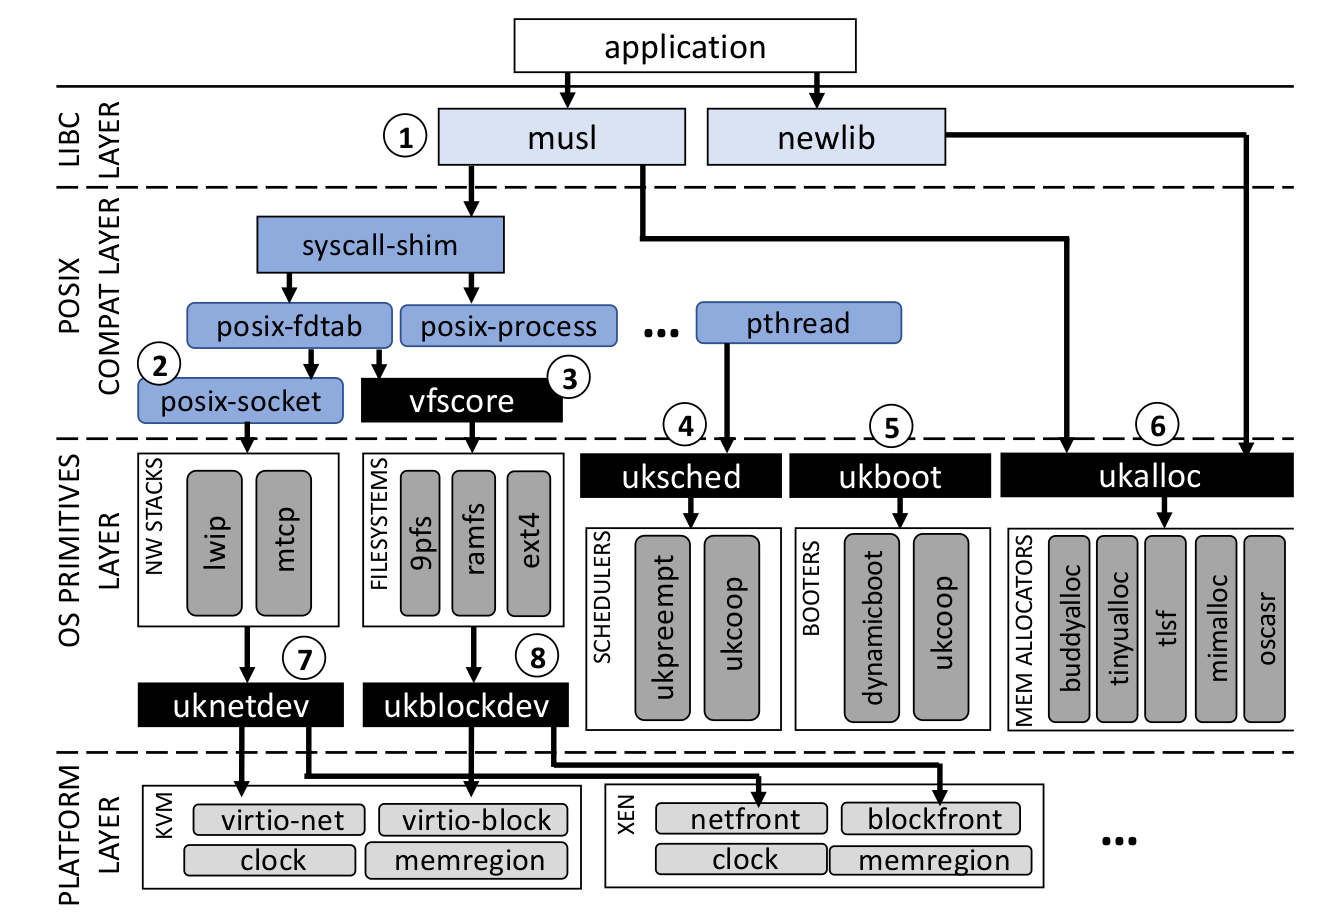
\includegraphics[width=\linewidth]{assets/Unikraft-architecture.png}
\caption{Unikraft的架构}\label{fig:unikraft-arch}
\end{minipage}
\begin{minipage}{0.49\linewidth}
\centering
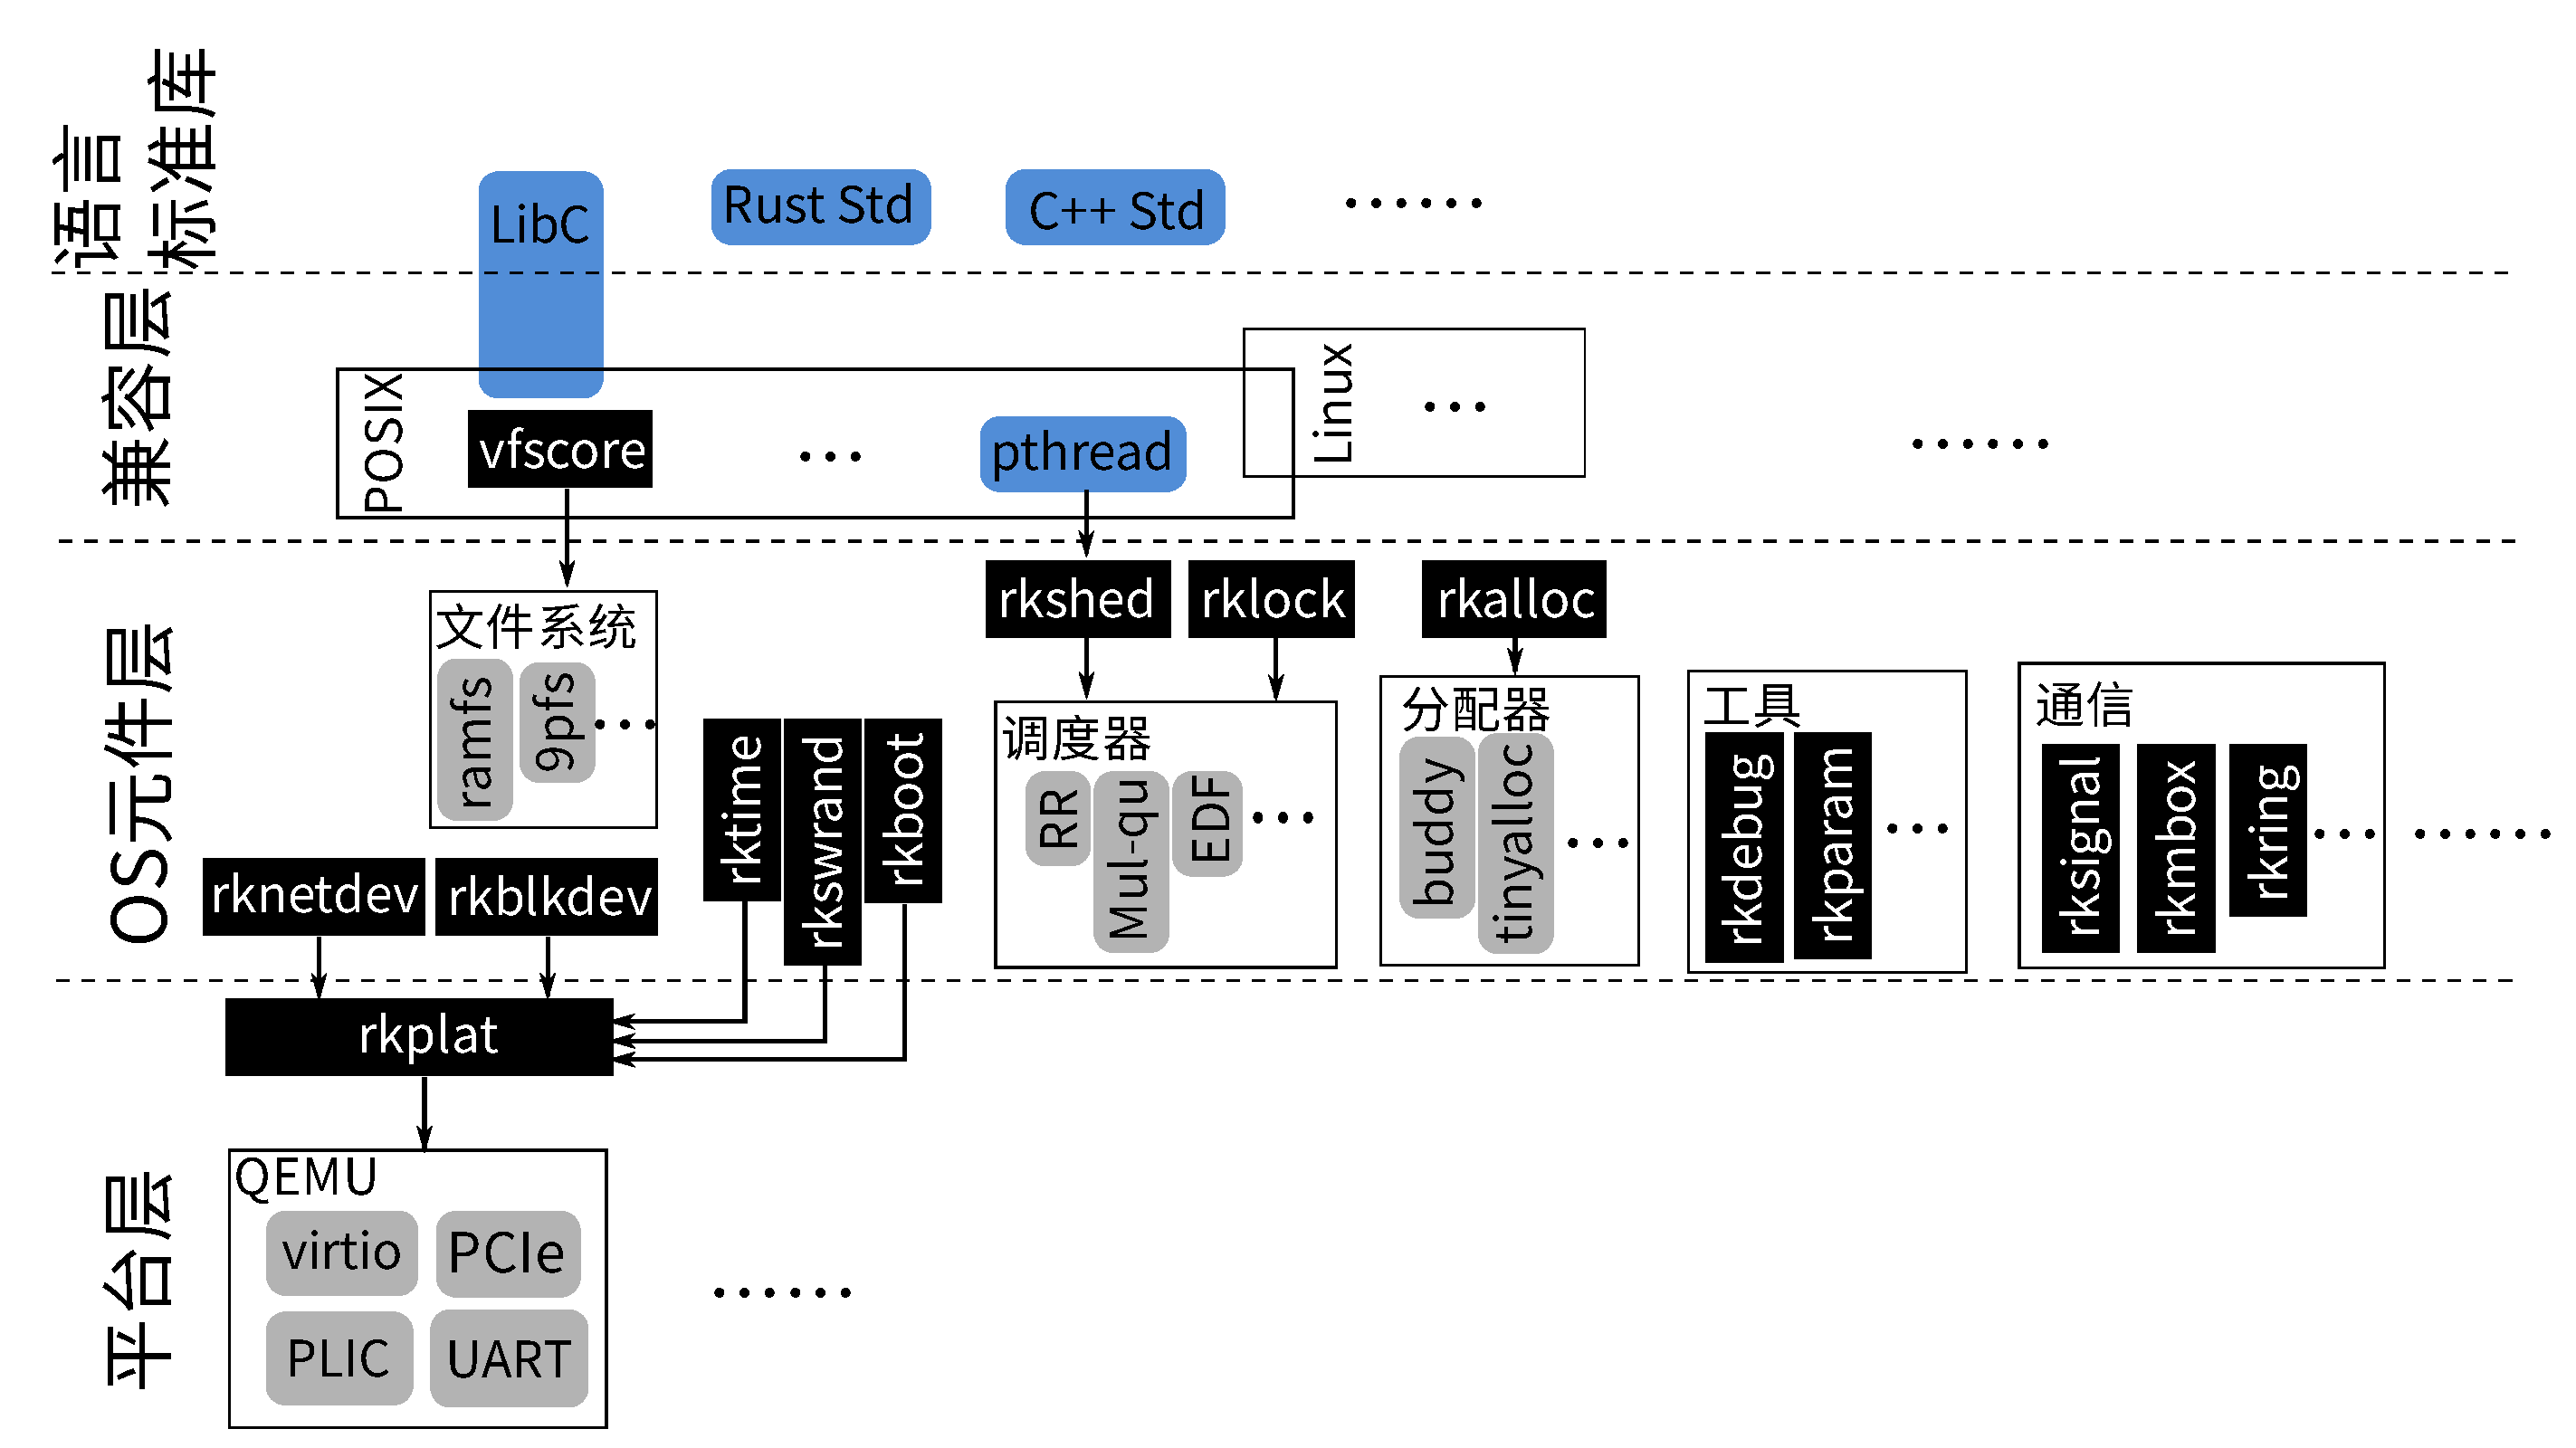
\includegraphics[width=\linewidth]{assets/Runikraft-architecture.pdf}
\caption{Runikraft的架构}\label{fig:runikraft-arch}
\end{minipage}
\end{figure}
平台层将不同的平台封装成通用的\texttt{rkplat} API,它提供与平台/架构密切相关的功能,
比如外设驱动、外中断处理、内存分页、定时器、原子操作、内存屏障,我们只计划支持RISC-V+QEMU virt
一种平台。如果时间不足,我们可以将现成的OpenSBI\cite{5}\cite{6}封装成\texttt{rkplat} API。

\texttt{rknetdev}、\texttt{rkblkdev}、\texttt{rktime}、\texttt{rkswrand}、\texttt{rkboot}
五个APIs的功能与平台密切相关,
但是为了降低开发和维护难度,它们并没有直接实现,而是在\texttt{rkplat}提供的初级抽象的基础上实现。
\texttt{rknetdev}和\texttt{rbblkdev}对应图\ \ref{fig:unikraft-arch}\ 的⑦和⑧,
它们分别提供网络设备和块设备的支持。
%与Unikraft的实现类似,这两个APIs的构造函数的参数接受指向\texttt{trait RKplat}的指针。
\texttt{rktime}提供获取和修改系统时间的API,\texttt{rkswrand}提供密码学安全的随机数,
\texttt{rkboot}负责完成系统的初始化并将控制权转交给用户的代码。

\texttt{rkshed}和\texttt{rklock}是两个与调度器有关的APIs,前者负责创建、调度、撤销线程,后者负责线程间
的同步和互斥。Runikraft支持多种调取器,比如,图\ \ref{fig:runikraft-arch}\ 中的RR的时间片轮转调度器、
Mul-qu是多重队列调取器、EDF是截止日期有限调度器。我们计划先实现RR调度器。当然,为了系统镜像的轻量性,
用户可以不使用任何调取器,这时,\texttt{rkshed}和\texttt{rklock}会被编译成空API,创建线程的行为
将和函数调用相同。这保证了大部分使用仅仅并行加速的程序仍然能正确运行。

Runikraft选择性地提供线程通信模块,如UNIX风格的信号(\texttt{rksignal}),信箱(\texttt{rkmbox}),
无锁的环形缓冲队列(\texttt{rkring})。

我们目前没有计划区分线程和进程,Runikraft的线程同时具有传统的OSes的线程和进程的特性:
线程之间没有隔离措施,但是线程之间又可以使用进程通信的方法更安全地同步。

\texttt{rkalloc}是分配器API,它的后端可以是\texttt{buddy}、\texttt{tinyalloc}、\texttt{tlsf}、
\texttt{mimalloc}等分配器。
不过,我们可能只会实现其中的一个。

Runikraft还提供了一些工具模块,比如调试工具\texttt{rkdebug}、命令行参数分析工具\texttt{rkparam}。

在 Unikraft 中,文件系统 API vfscore 是 POSIX 兼容层的一部分,我们沿用了它的设
计,将 \texttt{vfscore} 放在了兼容层。Runikraft计划支持RAM上的临时文件系统和Plan 9 OS的9fps。

位于最顶层的是语言标准库,这一层可以帮助Runikraft支持多种语言。
虽然语言标准库层被画在了兼容层之上,但它其实是直接用OS元件层的APIs实现的,这能避免分层系统
的低效。
我们只打算实现Rust标准库和C标准库的部分内容。


\section*{许可协议}
本文档以知识共享署名 4.0 国际 (CC BY 4.0)许可证发布。

\vspace{2ex}
\noindent\textbf{\large 您可以自由地}:
\begin{description}
\item[共享] 在任何媒介以任何形式复制、发行本作品;
\item[演绎] 修改、转换或以本作品为基础进行创作
在任何用途下,甚至商业目的。
\end{description}

\vspace{2ex}
\noindent\textbf{\large 惟须遵守下列条件}:
\begin{description}
\item[署名] 您必须给出适当的署名,提供指向本许可协议的链接,
同时标明是否(对原始作品)作了修改。您可以用任何合理的方式来署名,
但是不得以任何方式暗示许可人为您或您的使用背书。
\item[没有附加限制] 您不得使用法律术语或者技术措施,从而限制其他人
做许可协议允许的事情。
\end{description}

\vspace{2ex}
\noindent\textbf{\large 声明}:

您不必因为公共领域的作品要素而遵守许可协议,或者您的使用被可适用的例外或限制所允许。

不提供担保。许可协议可能不会给与您意图使用的所必须的所有许可。
例如,其他权利比如形象权、隐私权或人格权可能限制您如何使用作品。

本许可证的全文位于:\\
\centerline{\url{https://creativecommons.org/licenses/by/4.0/legalcode.zh-Hans}}
\bibliographystyle{IEEEtran}
\bibliography{feasibility-report}
\end{document}